\section{Model Formulation and Solution for Problem 3}

\subsection{Model Formulation}

Problem 3 fixes the specified AI and non-AI IT loads without altering job regions or start times. Only renewable allocation, storage charging and discharging, and grid transactions are optimized, isolating the energy-side contribution of storage.

Let $F_{rt}$ denote the facility load in region $r$ during period $t$,
$P^{RE}_{rt}$ the available renewable power,
and $B_{rt}$ the grid purchase power.
Direct renewable supply, renewable charging, grid charging, storage discharge,
renewable exports, and curtailment are denoted by
$V_{rt}$, $C^{RE}_{rt}$, $C^G_{rt}$,
$D_{rt}$, $X_{rt}$, and $R_{rt}$, respectively.
Facility loads and hourly energy balances satisfy
\begin{equation}
	\begin{aligned}
		F_{rt}
		&=
		PUE_r
		\left(
		P^{AI}_{rt}+P^{NonAI}_{rt}
		\right),\\
		P^{RE}_{rt}
		&=
		V_{rt}+C^{RE}_{rt}+X_{rt}+R_{rt},\\
		B_{rt}+V_{rt}+D_{rt}
		&=
		F_{rt}+C^G_{rt}.
	\end{aligned}
	\label{eq:q3_energy_balance}
\end{equation}

Here $F_{rt}$ is known, with $0\leq V_{rt}\leq F_{rt}$ and $0\leq C^G_{rt}\leq B_{rt}$.

Let $S_{rt}$ denote stored energy at the start of period $t$. Data-center storage scheduling typically uses SOC dynamics and power limits for intertemporal regulation\cite{ref10}. We additionally impose mutually exclusive charging and discharging, grid transaction limits, and terminal SOC constraints in a full-horizon optimization.
The time step is 1 h, with charging and discharging efficiencies $\eta_r^c$ and $\eta_r^d$,
giving the SOC recursion
\begin{equation}
	S_{r,t+1}
	=
	S_{rt}
	+
	\eta_r^c
	\left(
	C^{RE}_{rt}+C^G_{rt}
	\right)
	-
	\frac{D_{rt}}{\eta_r^d}.
	\label{eq:q3_soc}
\end{equation}

Storage satisfies capacity and power limits and $S_{r,2406}\geq S_{r0}$. Introduce $y_{rt}\in\{0,1\}$ to exclude simultaneous charging and discharging:
$C^{RE}_{rt}+C^G_{rt}\leq y_{rt}P_r^{ch,\max}$,
$D_{rt}\leq(1-y_{rt})P_r^{dis,\max}$.
Purchases satisfy $0\leq B_{rt}\leq P_r^{Grid,\max}$; renewable exports satisfy $0\leq X_{rt}\leq\bar X_r$ and $X_{rt}\leq P_r^{Grid,\mathrm{out},\max}$.

Cost and emissions follow Problem 2, with additional metrics for peak net grid purchases and net purchase fluctuations.
Define regional net purchase power as $N_{rt}=B_{rt}-X_{rt}$.
Then
\begin{equation}
	\begin{aligned}
		C&=
		\sum_r\sum_t
		\left(
		\pi_{rt}B_{rt}-\sigma_{rt}X_{rt}
		\right),\\
		E&=
		\sum_r\sum_t
		\kappa_{rt}B_{rt},\\
		P&=
		\sum_rP_r^{\max},
		\qquad
		P_r^{\max}\geq N_{rt},\quad
		P_r^{\max}\geq0,\\
		W&=
		\frac{1}{6(T-1)}
		\sum_r\sum_tW_{rt}.
	\end{aligned}
	\label{eq:q3_objectives}
\end{equation}

Here $t=0,\ldots,2405$ and $T=2406$, with $W_{rt}\geq\pm(N_{r,t+1}-N_{rt})$. Thus $W$ is the mean absolute change in net purchases between adjacent hours. The constraint $P_r^{\max}\geq0$ prevents net exports from being interpreted as negative peaks.

The four metrics have different units and no prescribed weights. First compute the single-objective ideal values $f_m^{best}$, evaluate each single-objective schedule $x^{(j)}$ on all metrics, and set $f_m^{ref}=\max_j f_m(x^{(j)})$.
For metrics with an effective trade-off range, define
\begin{equation}
	\bar f_m
	=
	\frac{f_m-f_m^{best}}
	{f_m^{ref}-f_m^{best}}.
	\label{eq:q3_normalization}
\end{equation}

If $f_m^{ref}=f_m^{best}$, the metric is used only for evaluation. Remaining metrics enter three-level selection:
\begin{equation}
	\begin{aligned}
        &\text{Level 1:}\quad
		\min z,
		\qquad
		\bar f_m\leq z;\\
        &\text{Level 2:}\quad
		\min \Phi=\sum_m\bar f_m;\\
        &\text{Level 3:}\quad
		\min G=
		\sum_r\sum_t
		\left(
		C^{RE}_{rt}+C^G_{rt}+D_{rt}
		\right).
	\end{aligned}
	\label{eq:q3_multilevel}
\end{equation}

The first two levels control maximum and total deviations. The third reduces unnecessary cycling among nearly equivalent schedules. All constraints except charge--discharge exclusivity are linear; the mixed-integer linear program is solved over hours 0--2405, with terminal SOC checked at 2406.


\subsection{Results and Model Validation}

Figure~\ref{fig:q3_storage} gives the unified six-region solution: RegionA--RegionC show almost no charging or discharging, while regulation is concentrated in RegionD--RegionF.
SOC in RegionD ranges approximately from $90.0\sim712.4$ MWh,
and the corresponding ranges in RegionE and RegionF are
$82.0\sim820.0$ MWh and $85.0\sim850.0$ MWh,
consistent with the charge and discharge dynamics in Equation~(\ref{eq:q3_soc}).

\begin{figure}[H]
	\centering
	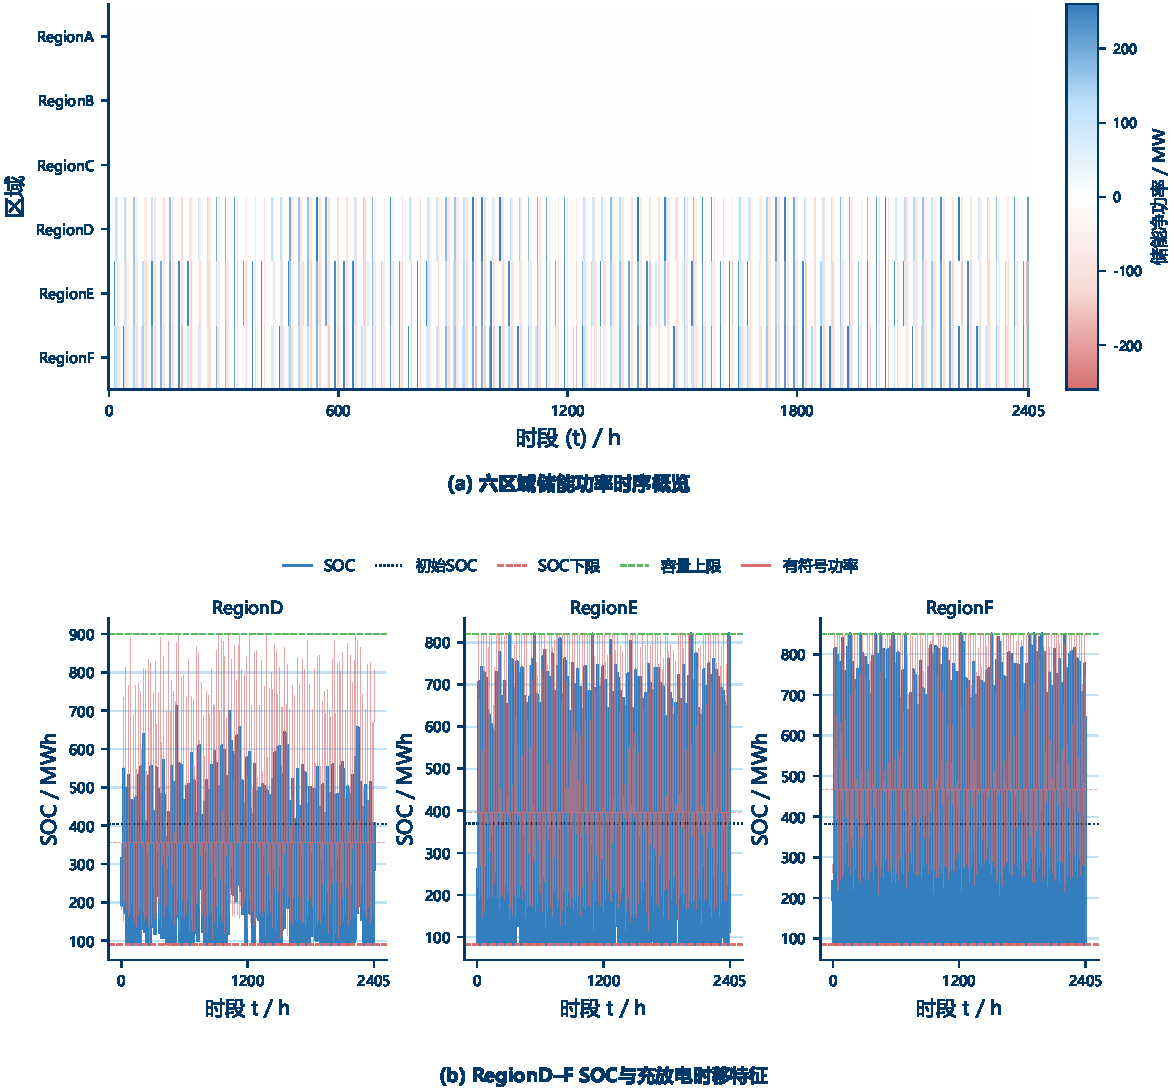
\includegraphics[width=0.92\textwidth]
	{figures/q3_group1_storage_mechanism.pdf}
    \caption{Storage power in six regions and SOC evolution in active regions}
	\label{fig:q3_storage}
\end{figure}

Storage is thus used mainly in regions with stronger regulation demand, rather than uniformly across regions.

The states supplied in the problem attachments are an operating reference only, not an optimization baseline in the same feasible set satisfying our terminal SOC condition. The no-storage schedule provides a model-consistent ablation.
The optimized operating cost is
$C=-4.5906\times10^{8}$,
with carbon emissions $E=0$,
the sum of six regional peak net purchases $P=0$,
and mean net purchase fluctuation $W=0.0113$ MW.
All four metrics improve on the attachment reference. Negative cost means export revenue exceeds purchase expenditure.

Zero emissions and peak net purchases do not imply zero data-center electricity load. Under the specified accounting rules, emissions arise only from grid purchases and the peak metric uses the positive part of net purchase power. For the present deterministic data and permitted renewable exports, renewables and storage supply the loads while surplus renewables are exported, reducing purchase-related emissions and positive net purchase peaks to zero. This depends on the current renewable, price, storage, and grid transaction conditions; zero values are not guaranteed under other parameter scenarios.

\begin{figure}[H]
	\centering
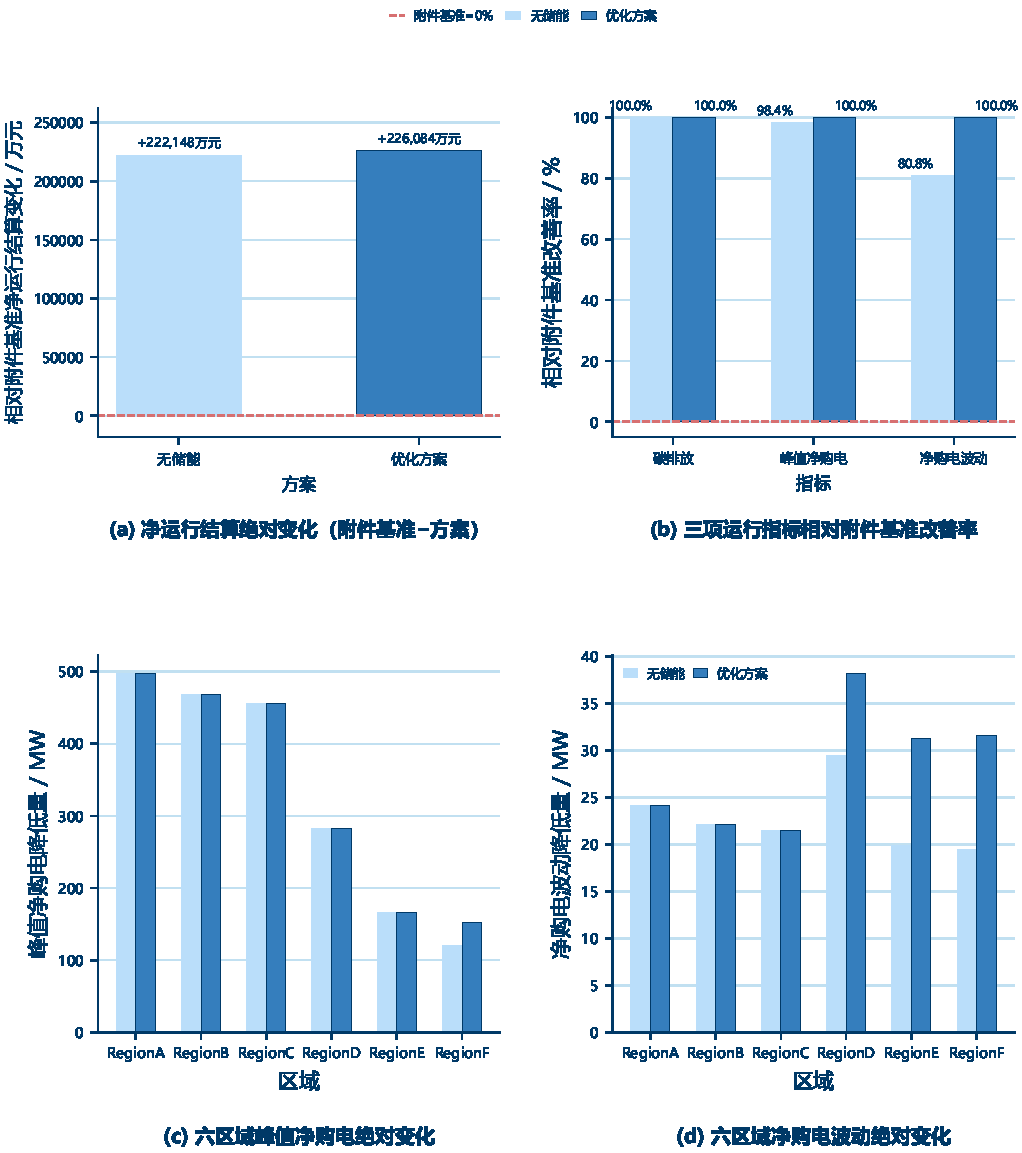
\includegraphics[width=0.86\textwidth]
{figures/q3_group2_optimization_effect.pdf}
\caption{Absolute net settlement changes, improvements in three metrics, and regional differences under storage coordination}
	\label{fig:q3_effect}
\end{figure}

Figure~\ref{fig:q3_effect} expresses absolute net settlement changes in CNY $10^4$ and the other metrics as relative improvements, avoiding ambiguous cost percentages when costs cross zero. All regional peaks fall; larger fluctuation improvements in RegionD--RegionF match the regions with active storage.

Set $C^{RE}_{rt}=C^G_{rt}=D_{rt}=0$ to construct a no-storage counterfactual.
Its operating cost is $-4.1969\times10^{8}$,
carbon emissions are $8.8506$,
peak net purchases are $31.5979$ MW,
and mean net purchase fluctuation is $5.3981$ MW.
Compared with this counterfactual, optimization reduces net operating cost by 3936.19 units of CNY $10^4$, as well as emissions, peaks, and fluctuations.

Independent verification confirms that both the optimized and no-storage schedules satisfy energy balance, SOC, capacity, exclusivity, grid transaction, and terminal constraints.
Maximum renewable and load balance residuals in the attachment operating reference are approximately
$2.0\times10^{-4}$ MW and $1.504\times10^{-4}$ MW,
consistent with the precision of the original data.
However, the maximum SOC recursion deviation is about $0.9999$ MWh,
and the terminal SOC deficit is approximately $193.3$ MWh.
The attachment states therefore serve as an operating reference, but are not a feasible optimization solution under our constraints.

\begin{figure}[H]
	\centering
	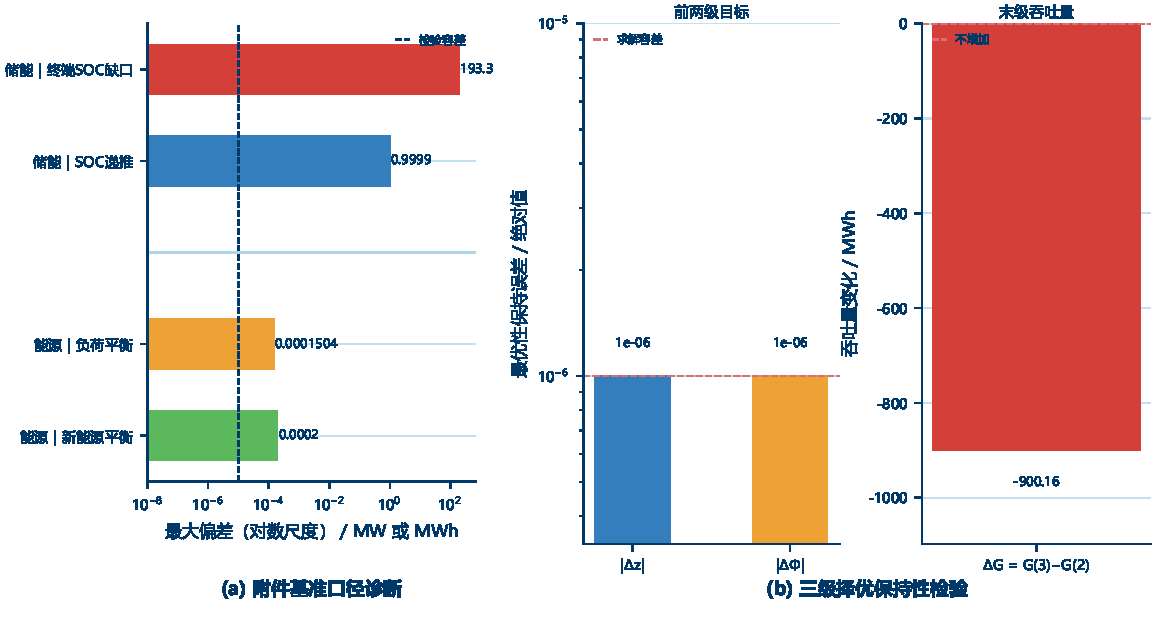
\includegraphics[width=0.91\textwidth]
	{figures/q3_group3_validation_credibility.pdf}
    \caption{Attachment-reference diagnostics and three-level multiobjective selection tests}
	\label{fig:q3_validation}
\end{figure}

In Figure~\ref{fig:q3_validation}, the third level changes $z$ and $\Phi$ by approximately $1.0\times10^{-6}$ relative to the preceding level while reducing storage throughput by 900.16 MWh. It reduces unnecessary cycling while retaining the first two levels' results.

Problem 3 quantifies intertemporal storage regulation under fixed loads and provides an energy-side baseline for Problem 4.



\section{Model Formulation and Solution for Problem 4}

\subsection{Model Formulation}

Problem 4 jointly optimizes job regions, start times, renewables, storage, and grid transactions. It initializes jobs with the feasible Problem 2 schedule and retains the energy mechanisms of Problem 3. Migration and time shifting affect renewable utilization, SOC, and grid exchanges through the PUE mapping, yielding a joint computing--storage--electricity model.

Spatial and temporal load shifting can coordinate with storage and electricity decisions\cite{ref9}. We retain deadlines, network latency, resource capacities, and energy limits, adding terminal SOC and rolling recoverability constraints.

The job-side feasible set follows Problem 1. Variables $x_{irs}$ and Equation~(\ref{eq:q1_overlap}) determine the AI IT load
$P_{rt}^{AI}=\sum_i\sum_{s\in S_i}p_i\rho_{ist}x_{irs}$,
and the facility load is
$F_{rt}=PUE_r(P_{rt}^{AI}+P_{rt}^{NonAI})$.
Each job executes exactly once. Real-time jobs start immediately; flexible jobs satisfy time windows, latency, GPU and power capacities, and the boundary at 2406.

The energy side retains Equations~(\ref{eq:q3_energy_balance}) and (\ref{eq:q3_soc}), their capacity, exclusivity, grid transaction, and export constraints, and $S_{r,2406}\geq S_{r0}$.

To prevent excessive early discharge in rolling optimization, an SOC recoverability condition is imposed at the end of each decision window:
\begin{equation}
	S_{r,\tau+H}
	\geq
	\max\left\{
	S_r^{\min},
	S_{r0}-
	\eta_r^cP_r^{ch,\max}(2406-\tau-H)
	\right\}.
	\label{eq:q4_soc_recovery}
\end{equation}

Equation~(\ref{eq:q4_soc_recovery}) preserves the theoretical ability to restore initial SOC within the remaining horizon and connects to the terminal constraint.

The six metrics are net operating settlement $C$, carbon emissions $E$, network latency $L$, waiting loss $J$, renewable nonutilization $Q$, and peak net purchases $P$. The first three follow Problems 2 and 3. Let $\underline{s}_i,\overline{s}_i$ denote valid start-time bounds for flexible jobs and $\omega_i$ latency-sensitive weights. Then
\begin{equation}
	\begin{aligned}
		J&=
		\frac{
			\displaystyle\sum_{i\in I^{\mathrm{flex}}_+}
			\omega_i
			\frac{s_i-\underline{s}_i}
			{\overline{s}_i-\underline{s}_i}}
		{\displaystyle\sum_{i\in I^{\mathrm{flex}}_+}\omega_i},
		\qquad QoS=1-J,\\
		Q&=
		\frac{\displaystyle\sum_r\sum_tR_{rt}}
		{\displaystyle\sum_r\sum_tP^{RE}_{rt}},
		\qquad U=1-Q,\\
		P&=\sum_rP_r^{\max},
		\qquad
		P_r^{\max}\geq B_{rt}-X_{rt},
		\quad P_r^{\max}\geq0.
	\end{aligned}
	\label{eq:q4_metrics}
\end{equation}

Global centers $a_m$ and scales $R_m$ are fixed before rolling optimization and remain unchanged across windows and scenarios. The nondegenerate active metric set is $\mathcal M_{\mathrm{act}}=\{L,J,Q\}$.
Normalized deviations and the augmented minimax criterion for window $\tau$ are
\begin{equation}
	\begin{aligned}
		d_{m,\tau}
		&=
		\max\left\{
		0,\,
		\frac{\hat f_{m,\tau}-a_m}{R_m}
		\right\},
		\qquad m\in\mathcal M_{\mathrm{act}},\\
		\min\quad Z_\tau
		&=
		z_\tau+\eta\sum_{m\in\mathcal M_{\mathrm{act}}} d_{m,\tau},
		\qquad
		d_{m,\tau}\leq z_\tau\quad(m\in\mathcal M_{\mathrm{act}}),
		\qquad
		\eta=10^{-3}.
	\end{aligned}
	\label{eq:q4_minmax}
\end{equation}

Equation~(\ref{eq:q4_minmax}) applies only to $\mathcal M_{\mathrm{act}}$. Metrics $C,E,P$ are independently recomputed for evaluation and scenario comparisons. All six form a common evaluation system, but they are not equally active optimization objectives.

The full-horizon joint integer model is too large. We use a rolling matheuristic initialized by the Problem 2 schedule, with $H=24$ h, $K=48$ h, and an internal advancement of 4 h. The look-ahead interval supplies future information only. Table~\ref{tab:q4_algorithm} summarizes the procedure.

\begin{table}[H]
	\centering
    \caption{Rolling joint computing--storage--electricity optimization for Problem 4}
	\label{tab:q4_algorithm}

	\fontsize{10.5pt}{12pt}\selectfont
	\renewcommand{\arraystretch}{0.88}

	\begin{tabular}{
			>{\centering\arraybackslash}p{0.08\textwidth}
			>{\raggedright\arraybackslash}p{0.86\textwidth}}
		\toprule
        \textbf{Step} & \multicolumn{1}{c}{\textbf{Operation}}\\
		\midrule

        1 & Read the Problem 2 seed schedule, current SOC, historical peaks, and remaining-job states.\\

        2 & Reoptimize storage and grid responses over the $H=24$ h decision window and $K=48$ h look-ahead interval.\\

        3 & Use marginal linear programs to assess the potential joint-objective effects of migrating or shifting flexible jobs.\\

        4 & Use small mixed-integer linear programs to repair local adjustments that create resource conflicts.\\

        5 & Form a large neighborhood of key jobs and jointly release job and energy variables for refinement.\\

        6 & Commit feasible decisions for the current $H$ hours; update SOC, historical peaks, cumulative emissions, and remaining jobs.\\

		\bottomrule
	\end{tabular}
\end{table}


The joint large neighborhood releases execution regions, start times, and energy variables together. It accepts only schedules satisfying every hard constraint and improving Equation~(\ref{eq:q4_minmax}). The result is a computationally efficient feasible schedule satisfying all hard constraints; global optimality is not claimed.

The sequential baseline fixes the Problem 2 job schedule and then optimizes storage and grid transactions using the Problem 3 energy model. Both schedules use the same six evaluation metrics.

Job, network, capacity, and storage parameters remain fixed while carbon constraints, pricing mechanisms, and renewable fluctuations vary. Let $E^0$ denote baseline emissions, $E^{LC}$ a low-carbon reference, and $\gamma$ a renewable smoothing parameter. The three scenario families are
\begin{equation}
	\begin{aligned}
		E
		&\leq
		E^0-\lambda(E^0-E^{LC}),
		\qquad 0\leq\lambda\leq1,\\
		\pi_{rt}^{fix}
		&=\bar{\pi}_r,
		\qquad
		\sigma_{rt}^{fix}=\bar{\sigma}_r,\\
		P_{rt}^{RE}(\gamma)
		&=
		(1-\gamma)P_{rt}^{RE}
		+\gamma\bar P_{rd}^{RE,+},
		\qquad
		t\in\mathcal H_{rd}^{+}.
	\end{aligned}
	\label{eq:q4_scenarios}
\end{equation}

Renewable smoothing applies only to originally nonzero periods and preserves daily total energy. All scenarios retain the fixed normalization scales.

Finally, the job table and complete SOC trajectories reconstruct profiles for hours 0--2405, allowing consistent recomputation of all six metrics and hard constraints.

\subsection{Results and Model Validation}

With $H=24$ h and $K=48$ h, 50000 jobs are processed through 101 rolling windows. Only decision-window results satisfying all hard constraints are committed, followed by full-horizon recomputation.

Degenerate reporting metrics in the earlier sequential energy solution produced a comparison baseline with limited physical meaning. To remove that effect, we fix both the Problem 2 sequential job schedule and the existing joint job schedule, then reoptimize storage and grid transactions using identical energy-response rules. This step consistently recomputes the two schedules' energy trajectories; it is not a rerun of the complete joint search. Table~\ref{tab:q4_result} gives the results.

\begin{table}[H]
	\centering
    \caption{Joint and sequential job schedules under consistent energy accounting}
	\label{tab:q4_result}

	\fontsize{10.5pt}{12pt}\selectfont
	\renewcommand{\arraystretch}{0.90}

	\begin{tabular}{lrr}
		\toprule
        \multicolumn{1}{c}{\textbf{Metric}}
        & \multicolumn{1}{c}{\textbf{Sequential jobs}}
        & \multicolumn{1}{c}{\textbf{Joint jobs}}\\
		\midrule

        Net settlement/CNY
		& $-4.532307\times10^8$
		& $-4.538873\times10^8$\\

        Emissions/tCO$_2$
		& 30.1233
		& 71.2005\\

        Mean network latency/ms
		& 12.9468
		& 9.9618\\

        QoS loss
		& 0.083659
		& 0.079281\\

        Renewable nonutilization
		& 29.8615\%
		& 29.8357\%\\

        Peak net purchases/MW
		& 66.5709
		& 97.1828\\

		\bottomrule
	\end{tabular}
\end{table}


In Table~\ref{tab:q4_result}, the joint job schedule lowers net settlement by $6.5665\times10^5$ CNY, latency by 2.9851 ms, QoS loss by 0.004378, and renewable nonutilization by 0.0258 percentage points. Emissions increase by 41.0772 tCO$_2$ and peak net purchases by 30.6119 MW. Negative settlement means export revenue exceeds purchase expenditure. Joint job adjustments mainly improve service quality and slightly reduce net settlement and curtailment; they do not improve all six metrics simultaneously.

The two schedules therefore cannot be ranked independently of decision preferences. A scheduler prioritizing latency, waiting loss, and renewable utilization while accepting increased emissions and peak purchases may choose the joint schedule. If emissions or peak purchases are strictly controlled, a schedule from the corresponding constrained scenario should be used. We interpret the results as feasible strategies for different operating preferences, rather than a unique optimum independent of application conditions.

\begin{figure}[H]
	\centering
	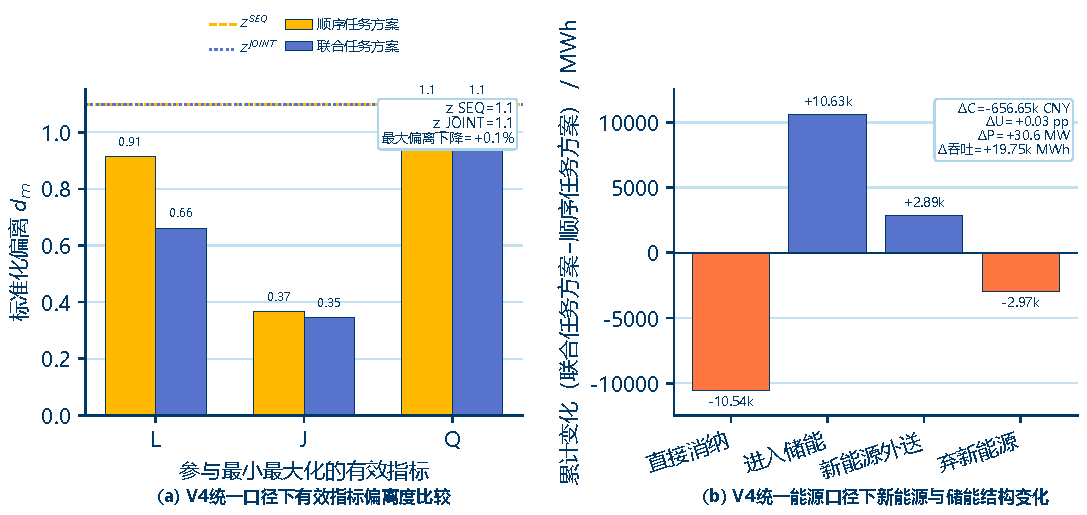
\includegraphics[width=0.88\textwidth]
	{figures/q4_group1_joint_optimization_results.pdf}
    \caption{Active metrics and renewable--storage structures of two job schedules under consistent energy accounting}
	\label{fig:q4_joint_result}
\end{figure}

In Figure~\ref{fig:q4_joint_result}, relative to sequential jobs, joint jobs reduce direct renewable use by $10.54\times10^3$ MWh, increase storage charging and exports by $10.63\times10^3$ and $2.89\times10^3$ MWh, reduce curtailment by $2.97\times10^3$ MWh, and increase storage throughput by $19.75\times10^3$ MWh. Metrics $L,J,Q$ are the nondegenerate active metrics actually used in the existing joint search. Metrics $C,E,P$ are independently recomputed with consistent energy accounting to report energy-side costs; they are not retrospectively described as joint-search objectives.

Equation~(\ref{eq:q4_scenarios}) defines carbon-constrained, fixed-price, and renewable-smoothing scenarios. Figure~\ref{fig:q4_scenario} shows changes relative to the joint baseline. It retains the completed scenario group and the joint baseline of that same version, comparing only within-group relative responses. Fixed-job energy recomputation in Table~\ref{tab:q4_result} and Figure~\ref{fig:q4_joint_result} specifically corrects the sequential--joint comparison. Absolute quantities from these two result groups are not combined.

\begin{figure}[H]
	\centering
	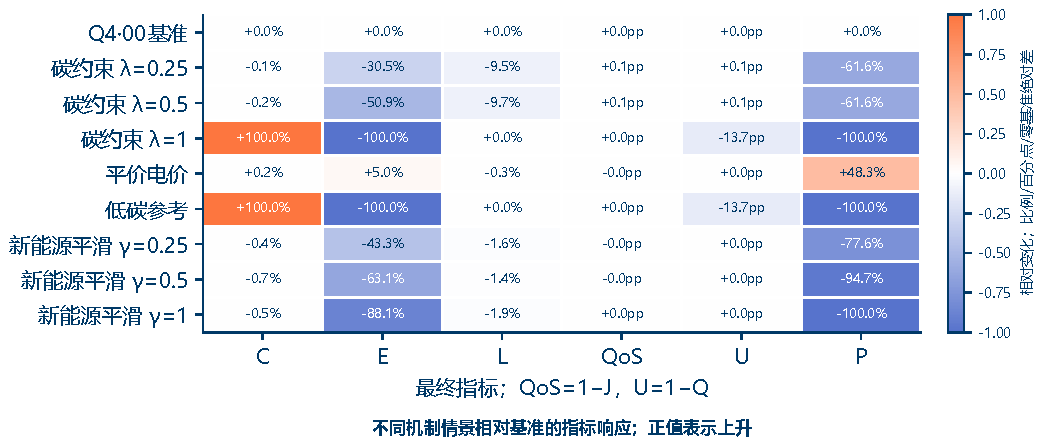
\includegraphics[width=0.86\textwidth]
	{figures/q4_group2_scenario_response.pdf}
    \caption{Scenario responses relative to the Problem 4 baseline}
	\label{fig:q4_scenario}
\end{figure}

In Figure~\ref{fig:q4_scenario}, increasing $\lambda$ from 0.25 to 0.50 lowers emissions from 297.36 to 209.97 tCO$_2$, with peaks around 95.54 MW and latency changing from 9.0144 to 8.9945 ms.
At $\lambda=1$, emissions and peak net purchases approach zero,
but renewable nonutilization rises to 43.5710\%.
Further restricting purchases therefore sacrifices renewable utilization rather than improving all metrics simultaneously.

Fixed electricity prices yield emissions of 449.37 tCO$_2$ and a peak of 368.71 MW. In renewable-smoothing scenarios,
for $\gamma=0.25,0.50,1.00$,
emissions are approximately 242.89, 158.01, and 50.85 tCO$_2$,
peak net purchases are approximately 55.73, 13.18, and 0 MW,
and latency remains within 9.77--9.81 ms. Smoothing mainly changes energy-side states.

Validation combines independent full-horizon recomputation with complete mixed-integer linear programs for representative windows. Both sequential and joint job schedules pass all 67 checks of jobs, capacity, latency, energy, SOC, and grid transactions. The largest hard-constraint violation is
$2.3842\times10^{-7}$, below the $10^{-6}$ verification tolerance.
The largest discrepancy between independently recomputed metrics and summary results is no greater than this order of magnitude.

\begin{figure}[H]
	\centering
	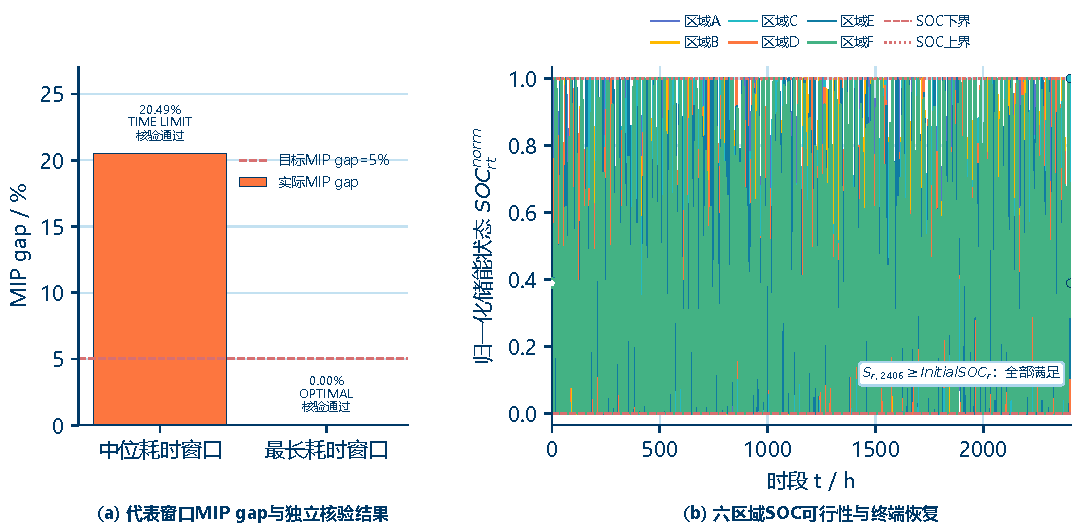
\includegraphics[width=0.88\textwidth]
	{figures/q4_group3_model_validation.pdf}
    \caption{Independent checks of complete representative-window mixed-integer models and six-region storage states}
	\label{fig:q4_validation}
\end{figure}

Figure~\ref{fig:q4_validation}(a) compares complete joint mixed-integer linear programs for windows 1512 and 2232. The former obtains a feasible reference with a 20.49\% relative gap within 600 s; the latter reaches optimality. Both pass constraint checks. This provides local feasibility and limited solution-quality references, not proof of full-horizon near-optimality or global optimality.

Figure~\ref{fig:q4_validation}(b) shows SOC trajectories for the joint job schedule after consistent energy recomputation. SOC stays within its bounds and satisfies $S_{r,2406}\geq S_{r0}$; benefits are not obtained by depleting initial stored energy.

Under the current data, the joint job schedule improves latency, waiting loss, and renewable nonutilization while increasing emissions and peak net purchases. Joint decisions therefore produce trade-offs rather than simultaneous superiority in all six metrics. Both schedules satisfy all job, computing, energy, and storage hard constraints. The conclusions concern computationally efficient feasible solutions; global optimality is not claimed, and fixed-job energy recomputation is not equated with complete joint search.
